\documentclass[aps, pre, reprint, amsmath, amssymb, superscriptaddress, floatfix]{revtex4-2}
\usepackage{ctex}
\usepackage{graphicx}
\usepackage{bm}
\usepackage{dcolumn}
\usepackage{hyperref}
\usepackage{xcolor}

\begin{document}

\title{皇后格点气体的统计力学：\\
从基态熵到平均场理论}

\author{Zong-Yue Liu}
\affiliation{Department of Physics, Nanjing University, Nanjing 210093, China}

\author{Lei Wang}
\affiliation{Institute of Physics, Chinese Academy of Sciences, Beijing 100190, China}

\date{\today}

\begin{abstract}
我们从统计力学的角度研究皇后格点气体——一种将 $M$ 个皇后放置在 $N \times N$ 棋盘上、沿共享行、列和对角线具有两两排斥相互作用的模型。在单位填充（$M = N$）条件下，基态恰好对应经典 $N$-皇后问题的 $Q(N)$ 个解，其熵 $s_0 \approx \ln N - \gamma$（$\gamma \approx 1.942$）与理想气体的 Sackur--Tetrode 公式具有引人注目的结构相似性，每个几何约束大约移除一个单位的熵。我们推导出精确的高温能量 $E/M \to 5/3$，并表明它分解为 $1/2 \times 2$（行和列）$+ 1/3 \times 2$（对角线），每个贡献可追溯到独立攻击线的占据统计。对 $N = 8$--$128$ 进行的大规模蒙特卡洛模拟（每个温度点 $10^8$ 次扫描）表明，每个皇后的比热 $C_v/M$ 在 $N \to \infty$ 时收敛到温度 $T$ 的普适函数，具有不发散的峰值 $C_v^{\max}/M \approx 1.62$（位于 $T^* \approx 0.237\,J$），从而确立了热力学相变的缺失。我们基于独立攻击线统计构建了修正泊松平均场理论，给出了极限情形下 $E/M(T)$ 和 $C_v/M(T)$ 的解析表达式，在 $T \ge 0.3\,J$ 时重现蒙特卡洛比热的误差在 $2\%$ 以内。对 $C_v/T$ 从 $T = \infty$ 到 $T = 0$ 的热力学积分恢复了已知的基态熵，提供了连接组合数学、模拟和热力学的非平凡自洽性检验。在半填充（$M = N^2/2$）条件下，能量标度为 $E \sim N^3$——与单位填充时的 $E \sim N$ 标度根本不同——系统表现出自平均性，每个皇后的能量涨落在热力学极限下消失（自平均）。
\end{abstract}

\maketitle

%=====================================================================
\section{引言}
\label{sec:intro}
%=====================================================================

$N$-皇后问题——在 $N \times N$ 棋盘上放置 $N$ 个互不攻击的皇后——是数学中最古老的组合问题之一，可追溯到 Bezzel 于 1848 年的工作~\cite{Bezzel1848}。尽管历史悠久，解的渐近计数直到最近才得以解决。Simkin~\cite{Simkin2022} 证明了解的数目 $Q(N)$ 满足
\begin{equation}
  Q(N) = \left((1 \pm o(1))\frac{N}{e^{\gamma}} \right)^N, \quad
  \gamma \approx 1.942,
  \label{eq:QN}
\end{equation}
这建立在 Bowtell 和 Keevash~\cite{Bowtell2023} 的突破以及 Luria 和 Simkin~\cite{Luria2021} 的早期界的基础上。常数 $\gamma$ 已通过数值方法精化~\cite{Nobel2023}。方程~\eqref{eq:QN} 给出每个皇后的基态熵
$s_0 = \lim_{N \to \infty} \ln Q(N)/N = \ln N - \gamma + o(1)$。

这一结果立即引发了统计力学的诠释。在本文中，我们设 $k_B = 1$，使得熵为无量纲量，温度具有能量单位。二维理想气体中 $N$ 个粒子在面积 $A$ 内的每粒子熵由 Sackur--Tetrode 公式给出~\cite{Reif1965}：
\begin{equation}
  s_{\rm gas} = \ln \frac{A}{N \lambda_{\rm th}^2} + 2,
  \label{eq:ST}
\end{equation}
其中 $\lambda_{\rm th} = h/\sqrt{2\pi m T}$ 是热 de Broglie 波长。两个表达式共享相同的函数形式：$\ln N$ 加上一个常数。在皇后系统中，每个皇后在其行内有 $N$ 个可能的列位置，因此
$\ln N$ 扮演了 $\ln\bigl(A/(N\lambda_{\rm th}^2)\bigr)$ 的角色：两者都表示每粒子可及"相空间"的对数。常数 $-\gamma$ 编码了施加几何约束的熵代价——类似于 Sackur--Tetrode 公式中由动量自由度和不可分辨性产生的常数 $+2$。

为使类比更加精确，我们注意到皇后问题可以分解为一系列约束严格程度递增的层次~\cite{Knuth2022}：
\begin{itemize}
  \item \textit{自由放置}（仅行约束）：
    $\Omega = N^N$，$s = \ln N$。
  \item \textit{排列}（行 + 列）：
    $\Omega = N!$，$s \approx \ln N - 1$。
  \item \textit{$N$-皇后}（行 + 列 + 两组对角线）：
    $\Omega \approx (N/e^\gamma)^N$，$s \approx \ln N - \gamma$。
\end{itemize}
列约束恰好消耗一个单位的熵（Stirling 近似修正）；两组对角线约束共消耗 $\gamma - 1 \approx 0.94$ 个单位，即每组对角线族约 $1/2$ 个单位。列排斥作为全局排列约束，每个粒子精确移除一个"比特"的自由度，而每组对角线族——其线段长度从 $1$ 到 $N$ 不等——大约移除半个单位。

受这种结构对应关系的启发，我们提出如下问题：皇后系统的有限温度热力学能否用解析方法理解？我们通过将 $N$-皇后问题嵌入具有可调温度的皇后格点气体~\cite{Zhang2009,Polson2024}，执行大规模蒙特卡洛模拟，并推导基于独立攻击线统计的泊松平均场理论——它提供了精度在百分之几以内的解析热力学描述——来回答这一问题。

皇后格点气体还与更广泛的约束满足问题（CSPs）领域相联系~\cite{Mezard2009,Krzakala2007}：单位填充时的 $N$-皇后问题恰好位于可满足性阈值处（$M \le N$：可解；$M > N$：冲突不可避免），类似于随机 $k$-SAT 在其临界子句密度附近的行为。

本文其余部分的组织如下。
第~\ref{sec:model}~节定义模型。
第~\ref{sec:entropy}~节详述熵与理想气体的类比。
第~\ref{sec:highT}~节推导高温极限。
第~\ref{sec:mc}~节展示 $M = N$ 的蒙特卡洛结果。
第~\ref{sec:mf}~节发展平均场理论。
第~\ref{sec:half}~节处理半填充情形 $M = N^2/2$。
第~\ref{sec:conclusions}~节为总结。


%=====================================================================
\section{模型}
\label{sec:model}
%=====================================================================

我们考虑具有开放边界条件的 $N \times N$ 正方格点。每个格点 $(i,j)$（$i,j = 1,\ldots,N$）携带一个占据变量 $n_{ij} \in \{0,1\}$。哈密顿量计数互相攻击的皇后对数：
\begin{equation}
  H = J \sum_{\langle (i,j),(i',j') \rangle_{\rm attack}}
  n_{ij}\, n_{i'j'},
  \label{eq:H}
\end{equation}
其中求和遍历所有共享同一行（$i = i'$）、同一列（$j = j'$）、同一主对角线（$i - j = i' - j'$）或同一反对角线（$i + j = i' + j'$）的格点对，且 $J > 0$。全文中设 $J = 1$。

格点自然分解为\textit{攻击线}：$N$ 条行、$N$ 条列、$2N-1$ 条主对角线和 $2N-1$ 条反对角线。
记 $n_\alpha$ 为攻击线 $\alpha$ 上的皇后数目，则哈密顿量取紧凑形式
\begin{equation}
  H = \sum_{\alpha \in \mathcal{L}} \binom{n_\alpha}{2},
  \label{eq:H_lines}
\end{equation}
其中 $\mathcal{L}$ 表示所有 $6N - 2$ 条攻击线的集合，$\binom{n}{2} = n(n-1)/2$ 计数每条线上的攻击对数。这种线贡献分解是高温计算（第~\ref{sec:highT}~节）和平均场理论（第~\ref{sec:mf}~节）的出发点。

我们在固定粒子数 $M = \sum_{ij} n_{ij}$ 的正则系综中工作，使用 Kawasaki 动力学~\cite{Kawasaki1966}（皇后-空位交换）和 Metropolis 准则~\cite{Metropolis1953}。一次\textit{扫描}包含 $M$ 次尝试交换。统计误差通过 200 个区间的 jackknife 重抽样估计~\cite{Efron1982}。对于 $M = N$ 的主要结果，我们模拟 $N = 8, 16, 32, 64, 100, 128$，每个温度点进行 $10^8$ 次测量扫描（318 个温度点，覆盖 $T = 0.05$ 到 $400\,J$），之前进行 $2 \times 10^6$ 次热化扫描，使用 32 个 CPU 并行计算。模型示意图及相关长度尺度示于图~\ref{fig:schematic}。

\begin{figure}[t]
  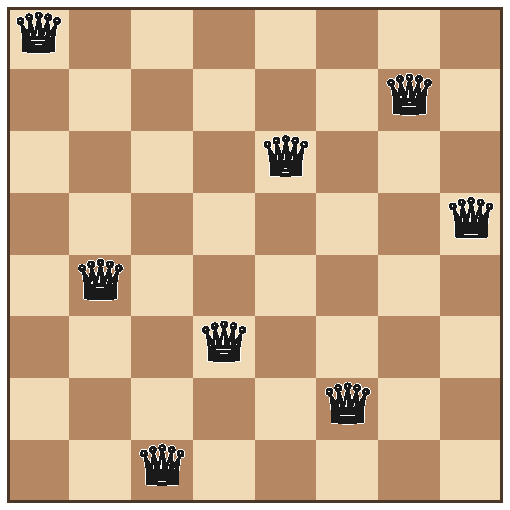
\includegraphics[width=\linewidth]{../figures/fig1_schematic.pdf}
  \caption{(a)~一个皇后（黑色圆圈）及其在 $8 \times 8$ 棋盘上的四条攻击线：行（红色）、列（蓝色）、主对角线（橙色）、反对角线（紫色）。(b)~$Q(8) = 92$ 个非攻击构型之一，$M = N = 8$ 个皇后。在理想气体类比中（第~\ref{sec:entropy}~节），物理棋盘边长 $L = N\lambda$ 扮演容器尺寸的角色，其中 $\lambda$（一个格点宽度）是类似于热 de Broglie 波长的格点间距，$\ln(L/\lambda) = \ln N$ 给出单粒子"相空间"熵。}
  \label{fig:schematic}
\end{figure}


%=====================================================================
\section{基态熵与理想气体类比}
\label{sec:entropy}
%=====================================================================

对于 $M = N$ 个皇后，基态（$E = 0$）对应 $Q(N)$ 个非攻击构型。利用方程~\eqref{eq:QN}，每个皇后的熵为
\begin{equation}
  s_0 = \frac{\ln Q(N)}{N}
  = \ln N - \gamma + o(1), \quad \gamma \approx 1.942.
  \label{eq:s0}
\end{equation}

三层约束层次（表~\ref{tab:entropy_levels}）提供了物理诠释。从完全无约束的模型出发，每个皇后独立选择 $N$ 列之一（$\Omega_{\rm free} = N^N$，$s_{\rm free} = \ln N$），列不重复约束将计数减少到 $N!$ 个排列。由 Stirling 近似 $\ln N! = N\ln N - N + O(\ln N)$，每个皇后的熵为
\begin{equation}
  s_{\rm perm} = \frac{\ln N!}{N}
  = \ln N - 1 + O\!\left(\frac{\ln N}{N}\right).
  \label{eq:s_perm}
\end{equation}
因此列约束恰好消耗一个单位的熵——即来自列分配不可分辨性的 Stirling 修正，与理想气体中的 Gibbs $1/N!$ 因子完全类比~\cite{Reif1965}。

两组对角线约束进一步将熵降低至 $s_0 = \ln N - \gamma$，额外消耗 $\gamma - 1 \approx 0.94$ 个单位，即每组对角线族约 $(\gamma - 1)/2 \approx 0.47$ 个单位。这一层次的代价在物理上是自然的：列约束作为 $N$ 条等价线上的全局排列，每个皇后精确移除一个单位的自由度，而每组对角线族——其线段长度从 $1$ 到 $N$ 不等——大约移除半个单位。

\begin{table}[b]
  \caption{$N$-皇后问题中逐步施加约束下每个皇后的熵。列约束恰好消耗 1 个单位；两组对角线约束共消耗 $\gamma - 1 \approx 0.94$ 个单位。}
  \label{tab:entropy_levels}
  \begin{ruledtabular}
  \begin{tabular}{llcc}
    模型 & 约束 & $\Omega$ & $s = \frac{1}{N}\ln\Omega$ \\
    \hline
    自由放置 & 仅行约束 & $N^N$ & $\ln N$ \\
    排列 & 行 + 列 & $N!$ & $\ln N - 1$ \\
    $N$-皇后 & 行 + 列 + 两组对角线 & $\approx (N/e^\gamma)^N$
      & $\ln N - \gamma$ \\
  \end{tabular}
  \end{ruledtabular}
\end{table}

与 Sackur--Tetrode 公式的结构对应关系现在变得明确。在二维理想气体中，$s_{\rm gas} = \ln(A/N\lambda^2) + 2$，其中对数项编码了每粒子的可及相空间，常数 $+2$ 来自两个动量自由度和 Gibbs 修正。对于皇后系统，$\ln N$ 是类似的"体积"项（每个皇后在其行内有 $N$ 个候选列），而 $-\gamma$ 是约束常数。自由气体与 $N$-皇后系综之间的全部差异为 $2 + \gamma \approx 3.94$ 个单位的熵，可追溯到五个"自由度"：两个动能（$p_x, p_y$），一个列排斥（Stirling/Gibbs），和两个对角线排斥。


%=====================================================================
\section{高温极限}
\label{sec:highT}
%=====================================================================

在 $T \to \infty$ 时，所有 $\binom{N^2}{M}$ 个包含 $M$ 个皇后的构型等概率。精确的高温能量可通过期望的线性性质得到~\cite{Polson2024}：将能量写为所有攻击格点对的求和，每对被占据的概率为 $M(M-1)/[N^2(N^2-1)]$（一个与对的位置无关的组合恒等式）。乘以攻击格点对总数 $S_{\rm tot} = N(N-1)(5N-1)/3$——其中 $N^2(N-1)/2$ 来自行，同等数目来自列，$N(N-1)(2N-1)/6$ 来自每组对角线族——给出对任意 $M$ 和 $N$ 的精确结果：
\begin{equation}
  \frac{\langle E \rangle}{M}\bigg|_{T \to \infty}
  = \frac{(5N-1)(M-1)}{3N(N+1)}.
  \label{eq:E_highT_general}
\end{equation}
对于单位填充 $M = N$，简化为
\begin{equation}
  \frac{\langle E \rangle}{M}\bigg|_{\substack{T \to \infty \\ M = N}}
  = \frac{(5N-1)(N-1)}{3N(N+1)}
  \xrightarrow{N \to \infty} \frac{5}{3}.
  \label{eq:E_highT}
\end{equation}

现在我们通过将能量分解为攻击线贡献来重新推导 $N \to \infty$ 的极限值 $5/3$，使用泊松近似揭示每一项的物理来源。

\subsection{行和列贡献}

考虑列贡献。在 $N^2$ 个格点上均匀随机放置 $M = N$ 个皇后时，每列的期望数目为 $M/N = 1$。这是一个经典的\textit{球进箱}问题：$N$ 个球（皇后）分配到 $N$ 个箱（列）中。在 $N \to \infty$ 极限下，任一给定列中的皇后数 $n_c$ 服从均值为 $\mu = M/N = 1$ 的泊松分布：
\begin{equation}
  P(n_c = k) = \frac{e^{-1}}{k!}, \quad k = 0, 1, 2, \ldots
  \label{eq:Poisson_col}
\end{equation}
一条列贡献的能量为 $\binom{n_c}{2} = n_c(n_c - 1)/2$。在泊松分布下的期望为
\begin{equation}
  \left\langle \binom{n_c}{2} \right\rangle
  = \frac{1}{2}\bigl(\langle n_c^2 \rangle - \langle n_c \rangle\bigr)
  = \frac{1}{2}(\mu^2 + \mu - \mu) = \frac{\mu^2}{2} = \frac{1}{2},
  \label{eq:col_energy}
\end{equation}
其中使用了泊松恒等式 $\langle n^2 \rangle = \mu^2 + \mu$。对 $N$ 条列求和再除以 $M = N$，得到每个皇后的列贡献为 $1/2$；行贡献由对称性完全相同。

\subsection{对角线贡献}

对于对角线，论证类似，但变化的对角线长度引入了积分。$N \times N$ 棋盘有 $2N - 1$ 条主对角线，长度为 $\ell = 1, 2, \ldots, N, \ldots, 2, 1$。长度为 $\ell$ 的对角线穿过 $N^2$ 个格点中的 $\ell$ 个。均匀随机放置 $M = N$ 个皇后时，该对角线上的期望皇后数为 $\mu_d = \ell \cdot M/N^2 = \ell/N$。每条对角线的期望碰撞能量为 $\langle\binom{n_d}{2}\rangle = \mu_d^2/2 = \ell^2/(2N^2)$，使用泊松结果。

对所有 $2N - 1$ 条主对角线求和再除以 $M = N$：
\begin{equation}
  \frac{E_{\rm diag}^+}{M} = \frac{1}{N} \sum_{d}
  \frac{\ell_d^2}{2N^2}.
  \label{eq:E_diag_sum}
\end{equation}
对于 $2N - 1$ 条主对角线，长度平方和为
$\sum \ell_d^2 = 2\sum_{k=1}^{N-1} k^2 + N^2 = N(2N^2+1)/3$。
因此
\begin{equation}
  \frac{E_{\rm diag}^+}{M}
  = \frac{1}{N} \cdot \frac{N(2N^2+1)}{6N^2}
  = \frac{2N^2+1}{6N^2}
  \xrightarrow{N \to \infty} \frac{1}{3}.
  \label{eq:E_diag_exact}
\end{equation}
等价地，在连续极限下，对角线长度用 $\mu = \ell/N \in (0, 1]$ 参数化，态密度为 $\rho(\mu) = 2N$（每个角处距离 $\mu$ 有两条对角线）。积分变为
\begin{equation}
  \frac{E_{\rm diag}^+}{M}
  \to 2\int_0^1 \frac{\mu^2}{2}\,d\mu = \frac{1}{3}.
  \label{eq:E_diag}
\end{equation}
包含两组对角线族，得到
\begin{equation}
  \frac{E}{M}\bigg|_{T \to \infty}
  = \underbrace{\frac{1}{2} + \frac{1}{2}}_{\text{行 + 列}}
  + \underbrace{\frac{1}{3} + \frac{1}{3}}_{\text{对角线}}
  = \frac{5}{3}.
  \label{eq:53}
\end{equation}

这一分解由蒙特卡洛模拟验证（图~\ref{fig:energy}）：在高 $T$ 时，$E/M$ 收敛到方程~\eqref{eq:E_highT} 给出的有限 $N$ 精确值，该值随 $N$ 增大从下方趋近 $5/3$，修正量为 $O(1/N)$ 量级。


%=====================================================================
\section{\texorpdfstring{$M = N$}{M=N} 的有限温度蒙特卡洛结果}
\label{sec:mc}
%=====================================================================

由于本节专注于单位填充 $M = N$，我们使用 $M$ 作为单一参数：$M \times M$ 棋盘上放置 $M$ 个皇后。

图~\ref{fig:energy} 展示了 $M = 8$--$128$ 的 $E/M$ 与 $T$ 的关系。$M \ge 32$ 的曲线几乎不可区分，确认了向热力学极限的快速收敛。

\begin{figure}[t]
  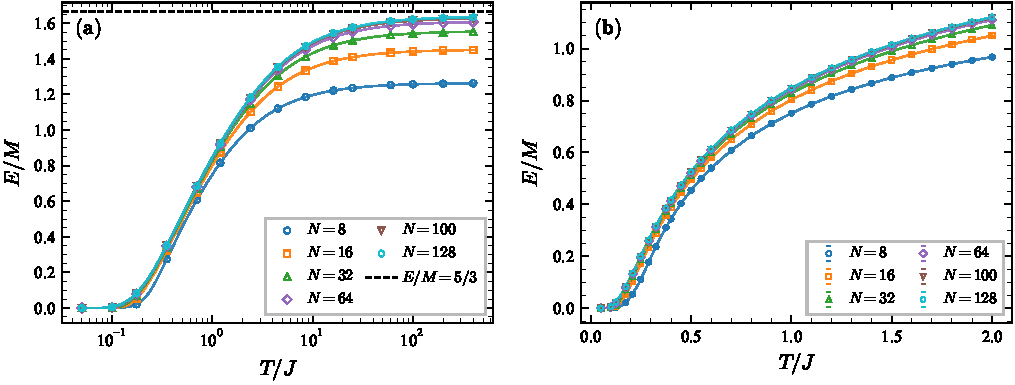
\includegraphics[width=\linewidth]{../figures/fig2_energy.pdf}
  \caption{不同 $N = 8$--$128$ 下每个皇后的能量 $E/M$ 与温度的关系。(a)~对数温度标度，覆盖全部范围 $T = 0.05$--$400\,J$；虚线标记 $N \to \infty$ 时的解析高温极限 $E/M = 5/3$。(b)~线性标度，放大至 $T \le 2\,J$，附误差棒。}
  \label{fig:energy}
\end{figure}

\subsection{比热收敛}

每个皇后的比热 $C_v/M = (\langle E^2\rangle - \langle E\rangle^2)/(T^2 M)$ 示于图~\ref{fig:cv}。对于 $M \ge 32$，$C_v/M$ 曲线坍缩到 $T$ 的单一函数上，表明已达到热力学极限。
表~\ref{tab:cv_peak} 列出了峰值。

\begin{figure}[t]
  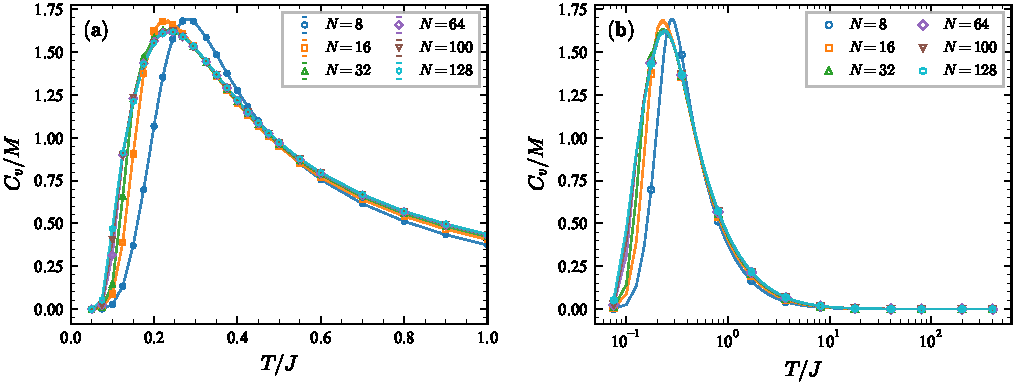
\includegraphics[width=\linewidth]{../figures/fig3_cv.pdf}
  \caption{$M = N$ 时每个皇后的比热 $C_v/M$ 与 $T$ 的关系。
  (a)~峰值区域（$T \le 1\,J$，线性标度），附误差棒。
  (b)~对数 $T$ 标度下的全温度范围。
  $M \ge 32$ 的曲线坍缩到单一函数上，确认了向热力学极限的收敛。}
  \label{fig:cv}
\end{figure}

\begin{table}[b]
  \caption{$M = N$ 时 $C_v/M$ 峰值的标度行为，由四次多项式拟合结合 bootstrap 重抽样（5000 次）确定。峰值高度在 $M \ge 32$ 时趋于饱和，约为 1.62，排除了发散的感生率从而排除了连续相变。}
  \label{tab:cv_peak}
  \begin{ruledtabular}
  \begin{tabular}{rD{.}{.}{3}D{.}{.}{4}D{.}{.}{4}}
    $M$ & \multicolumn{1}{c}{$T_{\rm peak}$}
    & \multicolumn{1}{c}{$C_v^{\max}/M$}
    & \multicolumn{1}{c}{误差} \\
    \hline
    8   & 0.281 & 1.6915 & 0.0002 \\
    16  & 0.227 & 1.6783 & 0.0006 \\
    32  & 0.231 & 1.6288 & 0.0005 \\
    64  & 0.237 & 1.6216 & 0.0004 \\
    100 & 0.237 & 1.6229 & 0.0004 \\
    128 & 0.237 & 1.6225 & 0.0004 \\
  \end{tabular}
  \end{ruledtabular}
\end{table}

关键观察是 $C_v^{\max}/M$ 在 $M \ge 32$ 时趋于饱和约 $1.62$，且\emph{不}随系统尺寸发散。这排除了热力学相变，并将该交叉行为认定为 Schottky 反常~\cite{Binder1997}——一种由有限能隙上的热激发引起的 $C_v$ 宽峰，无任何对称性破缺。峰值温度 $T^* \approx 0.237\,J$ 在 $M \ge 64$ 时稳定，峰值高度从上方单调收敛：$M = 64$ 与 $M = 128$ 之间的残余有限尺寸修正仅为 $\Delta C_v^{\max}/M \approx 0.001$，完全在统计误差棒范围内。

\subsection{熵的自洽性检验}
\label{sec:entropy_check}

$C_v/M$ 收敛到确定函数的性质使得一个强有力的热力学自洽性检验成为可能。我们通过两条独立途径计算 $T = \infty$ 与 $T = 0$ 之间的熵差。

\textit{组合途径。}---在 $T \to \infty$ 时，所有构型等概率，每个皇后的熵为
\begin{equation}
  \frac{S(\infty)}{M}
  = \frac{1}{M}\ln\binom{M^2}{M}.
  \label{eq:Sinf_def}
\end{equation}
当 $M \ll M^2$ 时，应用 Stirling 近似
$\ln n! = n\ln n - n + \tfrac{1}{2}\ln(2\pi n) + O(n^{-1})$：
\begin{align}
  \ln\binom{M^2}{M}
  &= \ln(M^2!) - \ln M! - \ln(M^2 - M)! \notag\\
  &= M\ln M - (M^2{-}M)\ln(1{-}1/M)
  + \Delta_{\rm S},
  \label{eq:Sinf_stirling}
\end{align}
其中前两项来自 Stirling 公式的 $n\ln n - n$ 部分，修正项
$\Delta_{\rm S} = \tfrac{1}{2}\ln[M^2/(2\pi M(M^2-M))]
= -\tfrac{1}{2}\ln(2\pi(M-1))$ 收集了次主导对数项。
展开 $\ln(1 - 1/M) = -1/M - 1/(2M^2) - \cdots$，主导项给出 $-(M^2-M)\ln(1-1/M) = M - \tfrac{1}{2} + O(M^{-1})$，因此
\begin{equation}
  \frac{S(\infty)}{M}
  = \ln M + 1 + O\!\left(\frac{\ln M}{M}\right).
  \label{eq:Sinf}
\end{equation}
在 $T = 0$ 时，只有基态贡献：
$S(0)/M = \ln Q(M)/M \approx \ln M - \gamma$。

\textit{热力学途径。}---基本关系
\begin{equation}
  S(\infty) - S(0) = \int_0^\infty \frac{C_v}{T}\,dT
  \label{eq:thermo_int}
\end{equation}
将熵差与比热联系起来。两边除以 $M$ 并代入上述结果：
\begin{equation}
  \int_0^\infty \frac{C_v}{MT}\,dT
  = \frac{S(\infty) - S(0)}{M}
  = 1 + \gamma + O\!\left(\frac{\ln M}{M}\right)
  \approx 2.94.
  \label{eq:DS}
\end{equation}
这是一个引人注目的关系：左边涉及通过模拟在整个温度范围内测量的 $C_v(T)$，而右边仅涉及\emph{组合}常数 1（来自 Stirling 近似修正）和 $\gamma$（来自 Simkin 渐近公式）。

对我们蒙特卡洛 $C_v$ 数据（每温度 $10^8$ 次扫描，318 个点覆盖 $T = 0.05$--$400\,J$）的数值积分给出的熵差 $\Delta S/M = \int_0^\infty (C_v/MT)\,dT$ 与该预言一致（表~\ref{tab:entropy_check}）。
对于 $M = 8$ 和 $M = 16$，$Q(N)$ 的精确值是已知的（$Q(8) = 92$，$Q(16) = 14\,772\,512$），因此 $S(0)/M$ 无需近似即可精确计算；低于百分之一的吻合度验证了我们的模拟和积分过程。对于 $M \ge 32$，精确的 $Q(N)$ 未知，$S(0)/M$ 必须从 Simkin 渐近公式 $Q(N) \approx (N/e^\gamma)^N$ 估算。$M = 32$ 处的偏差（$4.0\%$）最大，是因为 Simkin 公式在所应用的最小 $N$ 处具有最大的相对误差：方程~\eqref{eq:QN} 中的 $o(1)$ 修正项在 $N = 32$ 时仍然可观，但随 $N$ 快速递减，这解释了 $M = 64$（$1.8\%$）、$100$（$1.4\%$）和 $128$（$0.7\%$）处不断改善的吻合。$\Delta S_{\rm MC}/M$ 随 $M$ 增大向渐近值 $1 + \gamma \approx 2.94$ 单调收敛，确认了所有三个要素之间的相互自洽性。

\begin{table}[b]
  \caption{通过热力学积分进行的熵验证。
  $\Delta S_{\rm theory}/M = [S(\infty) - S(0)]/M$ 由精确的 $S(\infty)/M = \ln\binom{N^2}{N}/N$ 和已知的 $S(0)/M = \ln Q/M$ 计算（$M \le 16$ 时精确；$M \ge 32$ 时使用 Simkin 渐近值）。$\Delta S_{\rm MC}/M = \int_0^\infty (C_v/MT)\,dT$ 通过蒙特卡洛数据的数值积分得到（$10^8$ 次扫描，318 个温度点，最高至 $T = 400\,J$）。}
  \label{tab:entropy_check}
  \begin{ruledtabular}
  \begin{tabular}{cD{.}{.}{3}D{.}{.}{3}c}
    $M$ & \multicolumn{1}{c}{$\Delta S_{\rm theory}/M$}
    & \multicolumn{1}{c}{$\Delta S_{\rm MC}/M$}
    & 吻合度 \\
    \hline
    8   & 2.211 & 2.218 & 0.3\% \\
    16  & 2.567 & 2.572 & 0.2\% \\
    32  & 2.844 & 2.729 & 4.0\% \\
    64  & 2.887 & 2.836 & 1.8\% \\
    100 & 2.905 & 2.864 & 1.4\% \\
    128 & 2.912 & 2.891 & 0.7\% \\
  \end{tabular}
  \end{ruledtabular}
\end{table}

%=====================================================================
\section{平均场理论}
\label{sec:mf}
%=====================================================================

\subsection{物理图像}

$H$ 分解为攻击线贡献 [方程~\eqref{eq:H_lines}] 表明了一种自然的平均场近似：将不同攻击线上的占据数视为统计独立。在稀释极限 $M = N$ 下，密度 $\rho = M/N^2 = 1/N \to 0$，每个皇后属于四条攻击线，这些线不共享其他皇后的概率为 $1 - O(1/N)$。因此，任意\emph{一对}攻击线之间的关联为 $O(1/N)$，单独来看可以忽略。

然而，这并不使得该近似精确：每条长度为 $O(N)$ 的线与 $O(N)$ 条其他线各共享恰好一个格点，因此这些单独微弱的关联的\emph{累积}效应为
\begin{equation}
  \frac{\delta E}{M}
  \sim \frac{O(N)\text{ 条线} \times O(N)\text{ 个邻居} \times O(1/N)\text{ 每对}}{N}
  = O(1).
  \label{eq:mf_error}
\end{equation}
独立线近似因此给出的 $E/M$ 即使在 $N \to \infty$ 极限下也与真实值存在 $O(1)$ 量级的偏差——数值上为百分之几。尽管存在这一系统偏差，该近似仍捕获了正确的函数形式，并提供了定量有用的热力学描述。

\subsection{简单泊松平均场}

我们首先给出受文献~\cite{Polson2024} 启发的简单近似。每个皇后沿四族攻击线（行、列、主对角线、反对角线）相互作用，但这些族的约束强度不等：第~\ref{sec:entropy}~节的熵分析表明，每条行或列约束移除每个皇后一个单位的熵，而两组对角线约束共移除 $\gamma - 1 \approx 0.942$ 个单位。
因此我们分配一个\emph{熵加权}的有效相互作用方向数，
\begin{equation}
  \nu_{\rm eff} = \underbrace{1 + 1}_{\text{行 + 列}}
  + \underbrace{(\gamma - 1)}_{\text{两组对角线}} = 1 + \gamma
  \approx 2.942.
  \label{eq:nu_eff}
\end{equation}
将每个有效方向视为独立，并对每次冲突分配玻尔兹曼抑制
$e^{-J/(2T)}$（因子 2 来自两体能量在两个皇后间的平分），平均场每皇后能量为
\begin{equation}
  \frac{E^{\rm MF}}{M}
  = \frac{(1+\gamma)(N-1)}{2N}\,e^{-1/(2T)}
  \xrightarrow{N \to \infty}
  \frac{1+\gamma}{2}\,e^{-1/(2T)},
  \label{eq:E_simple}
\end{equation}
给出比热
\begin{equation}
  \frac{C_v^{\rm MF}}{M} = \frac{dE/M}{dT}
  = \frac{1+\gamma}{4T^2}\,e^{-1/(2T)}.
  \label{eq:Cv_simple}
\end{equation}
令 $dC_v/dT = 0$ 给出峰值位置 $T^* = 1/4$，对应
\begin{equation}
  \frac{C_v^{\max}}{M} = \frac{4(1+\gamma)}{e^2} \approx 1.593,
  \label{eq:Cv_peak_simple}
\end{equation}
与 $N = 128$ 的蒙特卡洛值 $1.615$ 相差 $1.4\%$。
残余偏差源于两种误差来源的部分抵消：熵加权前因子 $1+\gamma \approx 2.942$（而非完全的四族分解）带来的低估，以及忽略线间关联带来的高估。

\subsection{修正泊松平均场}

更系统的处理保留了四族攻击线（行、列、主对角线、反对角线）的完整分解，并考虑了变化的对角线长度。在有限温度下，均值为 $\mu$（在 $T = \infty$ 时）的攻击线上的占据数服从\textit{修正泊松分布}——一个由线内相互作用的玻尔兹曼因子重新加权的泊松分布。

对于具有逸度 $\lambda$、逆温度 $\beta = 1/T$ 的单条攻击线，找到 $k$ 个皇后的概率为
\begin{equation}
  P(n = k) = \frac{\lambda^k}{k!}\,
  e^{-\beta\,k(k-1)/2}\Big/\,g(\lambda, \beta),
  \label{eq:modPoisson}
\end{equation}
其中归一化配分函数为
\begin{equation}
  g(\lambda, \beta) = \sum_{k=0}^\infty
  \frac{\lambda^k}{k!}\,e^{-\beta k(k-1)/2}.
  \label{eq:g_def}
\end{equation}
逸度 $\lambda$ 由约束 $\langle n \rangle = \mu$ 自洽确定：
\begin{equation}
  \mu = \frac{\lambda}{g}\,\frac{\partial g}{\partial \lambda}
  = \sum_{k=0}^\infty k\,P(k).
  \label{eq:mu_constraint}
\end{equation}

方程~\eqref{eq:modPoisson} 的物理含义是透明的：$\lambda^k/k!$ 因子是线上 $k$ 个粒子的标准泊松权重，$e^{-\beta k(k-1)/2}$ 抑制具有多次碰撞的构型。在 $\beta = 0$（$T \to \infty$）时，$P(k)$ 退化为标准泊松分布；在 $\beta \to \infty$（$T \to 0$）时，只有 $k = 0$ 和 $k = 1$ 存在，强制执行非攻击约束。

每条线的期望碰撞能量为
\begin{equation}
  f(\mu, \beta) = \left\langle\binom{n}{2}\right\rangle
  = \frac{1}{2}\sum_{k=2}^{\infty} k(k-1)\,P(k).
  \label{eq:f_def}
\end{equation}

热力学极限下每个皇后的能量为
\begin{equation}
  \frac{E}{M}(T) = \underbrace{2\,f\!\left(1,\tfrac{1}{T}\right)
  }_{\text{行 + 列}}
  + \underbrace{4\int_0^1 f\!\left(\mu,\tfrac{1}{T}\right)d\mu
  }_{\text{对角线}},
  \label{eq:E_MF}
\end{equation}
其中第一项对 $N$ 条行和 $N$ 条列求和（每条 $\mu = 1$），积分项处理 $2 \times (2N-1)$ 条对角线（$\mu = \ell/N \in (0,1]$）。

\subsection{低温近似}

在低温（$\beta \gg 1$）时，配分函数 $g$ 由前几项主导。截断到 $k = 2$：
\begin{equation}
  g \approx 1 + \lambda + \frac{\lambda^2}{2}\,e^{-\beta}.
  \label{eq:g_trunc}
\end{equation}
注意 $k = 2$ 的玻尔兹曼因子为 $e^{-\beta \cdot 2(2-1)/2} = e^{-\beta}$，因为两个皇后共享一条线的能量代价为 $J = 1$。
对行/列贡献施加 $\langle n \rangle = 1$ 给出 $(\lambda^2/2)e^{-\beta} = 1$，因此 $\lambda = \sqrt{2}\,e^{\beta/2}$。
行 + 列每皇后能量为
\begin{equation}
  \frac{E_{\rm rc}}{M} \approx \frac{2}{2 + \sqrt{2}\,e^{\beta/2}},
  \label{eq:Erc_approx}
\end{equation}
具有二能级 Schottky 函数的形式。对应的比热贡献为
\begin{equation}
  \frac{C_{v,\rm rc}}{M} \approx
  \frac{\sqrt{2}\,e^{\beta/2}}{(2 + \sqrt{2}\,e^{\beta/2})^2}
  \cdot \frac{1}{T^2}.
  \label{eq:Cv_rc_approx}
\end{equation}
这一二能级（Schottky）近似正确捕获了峰形，并解释了比热为何不发散：能隙 $\Delta$ 是有限的，因此热激发始终是平滑的交叉行为而非临界现象。

\subsection{与蒙特卡洛的比较}

图~\ref{fig:mf} 将两种平均场预言与蒙特卡洛数据进行了比较。修正泊松理论系统性地高估 $E/M$ 约 $2$--$7\%$（低温端偏差较大）。如第~\ref{sec:mf}A~节所述，这一偏差是 $O(1)$ 量级的效应：每对攻击线通过共享格点产生 $O(1/N)$ 的关联，但 $O(N^2)$ 对这样的关联累积产生了在 $N \to \infty$ 极限下持续存在的修正。简单平均场由于误差抵消而偶然吻合良好。

对于比热，简单平均场给出 $C_v^{\max}/M = 4(1+\gamma)/e^2 \approx 1.593$（与 $N = 128$ 的蒙特卡洛值相差 1.4\%），修正泊松平均场给出 $1.692$（相差 4.8\%）。两者都正确预言了无发散及 Schottky 形状。平均场分解揭示，在 $C_v$ 峰值处，行 + 列贡献约 $67\%$，对角线贡献约 $33\%$ 的总比热。

表~\ref{tab:mf_comparison} 给出了在选定温度下 $N = 128$ 的详细比较。

\begin{table}[b]
  \caption{修正泊松平均场 vs.\ 蒙特卡洛（$N = 128$）。
  $E/M$ 的系统性高估是独立线近似忽略线间关联所致的 $O(1)$ 量级效应（见正文）。}
  \label{tab:mf_comparison}
  \begin{ruledtabular}
  \begin{tabular}{cD{.}{.}{5}D{.}{.}{5}cD{.}{.}{3}D{.}{.}{3}c}
    $T$ & \multicolumn{1}{c}{$E_{\rm MC}/M$}
    & \multicolumn{1}{c}{$E_{\rm MF}/M$}
    & $\Delta E$
    & \multicolumn{1}{c}{$C_{v,\rm MC}/M$}
    & \multicolumn{1}{c}{$C_{v,\rm MF}/M$}
    & $\Delta C_v$ \\
    \hline
    0.200 & 0.12064 & 0.12952 & 7.4\% & 1.554 & 1.646 & 5.9\% \\
    0.225 & 0.16034 & 0.17140 & 6.9\% & 1.615 & 1.692 & 4.8\% \\
    0.300 & 0.27974 & 0.29460 & 5.3\% & 1.520 & 1.550 & 2.0\% \\
    0.500 & 0.52559 & 0.54263 & 3.2\% & 0.973 & 0.976 & 0.3\% \\
    1.000 & 0.84800 & 0.86633 & 2.2\% & 0.436 & 0.439 & 0.7\% \\
  \end{tabular}
  \end{ruledtabular}
\end{table}

\begin{figure}[t]
  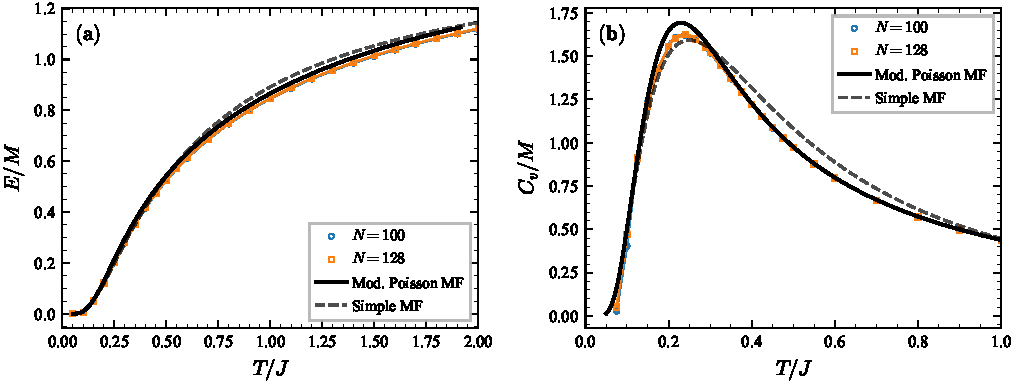
\includegraphics[width=\linewidth]{../figures/fig4_meanfield.pdf}
  \caption{$M = N$ 时平均场理论与蒙特卡洛的比较。
  (a)~$T \le 2\,J$ 范围内每个皇后的能量 $E/M$；实线为修正泊松平均场 [方程~\eqref{eq:E_MF}]，虚线为简单平均场。
  (b)~$T \le 1\,J$ 范围内的比热 $C_v/M$；两条平均场曲线都重现了峰形且无任何发散。仅展示最接近热力学极限的 $N = 100$ 和 $N = 128$ 蒙特卡洛数据。}
  \label{fig:mf}
\end{figure}


%=====================================================================
\section{半填充：\texorpdfstring{$M = N^2/2$}{M = N\^{}2/2}}
\label{sec:half}
%=====================================================================

现在转向高密度的另一极端，设 $M = N^2/2$。这一区域与稀释的 $M = N$ 情形根本不同：每行平均包含 $N/2$ 个皇后，每条线上的皇后对数目随 $N$ 广延增长。

\subsection{高温能量标度}

高温能量可通过与第~\ref{sec:highT}~节相同的球进箱分解推导。对于 $M = N^2/2$ 个皇后均匀放置在 $N^2$ 个格点上，每行的平均占据数为 $\mu_r = M/N = N/2$。每行的期望碰撞能量为 $\langle\binom{n_r}{2}\rangle = \mu_r^2/2 = N^2/8$（使用泊松近似，当 $M/N \to \infty$ 时在 $N \to \infty$ 极限下精确）。对 $N$ 行求和再除以 $M$ 给出每皇后行贡献 $(N \cdot N^2/8)/(N^2/2) = N/4$。加上列贡献（由对称性完全相同）得到 $E_{\rm rc}/M = N/2$。

对于对角线，长度为 $\ell$ 的对角线平均占据数为 $\mu_d = \ell M/N^2 = \ell/2$。求和并取连续极限：
\begin{equation}
  \frac{E_{\rm diag}}{M}
  = \frac{4N}{M}\int_0^1 \frac{(N\mu/2)^2}{2}\,d\mu
  = \frac{4N \cdot N^2}{8 \cdot N^2/2}\int_0^1 \mu^2\,d\mu
  = \frac{N}{3}.
  \label{eq:E_half_diag}
\end{equation}
合并：
\begin{equation}
  \frac{\langle E\rangle}{M}\bigg|_{T \to \infty}
  = \frac{N}{2} + \frac{N}{3} = \frac{5N}{6}.
  \label{eq:Ehalf}
\end{equation}
次主导修正给出精确结果 $(5N - 6)/6 + O(N^{-1})$~\cite{Polson2024}。
总能量 $E = M \cdot (5N/6) \sim N^3$ 使得这一区域与稀释情形（$E \sim N$）根本不同。与 Ising 模型在正方格点上的 $E \sim N^2$（在格点数目上广延）不同，这里的能量在 $N^2$ 上是\emph{超广延}的，反映了皇后相互作用的长程本质。

\subsection{自平均}

图~\ref{fig:half} 展示了 $N = 4$--$64$ 的蒙特卡洛结果。有两个值得注意的特征。首先，每皇后能量 $E/M$ 与 $N$ 成正比增长 [图~\ref{fig:half}(a)]，与方程~\eqref{eq:Ehalf} 一致。其次，比热峰变窄，每皇后幅度随 $N$ 减小 [图~\ref{fig:half}(b)]，表现出\textit{自平均}。

自平均是宏观可观测量在热力学极限下变为确定性量的现象，在无序系统中广为人知~\cite{Mezard1987}。在皇后格点气体中，它的出现是因为在半填充时每个皇后沿其攻击线与 $O(N)$ 个其他皇后相互作用，使得每皇后能量成为许多关联项的求和，其相对涨落随系统尺寸消失。定量地，固定 $T$ 下每皇后比热 $C_v/M$ 随 $N$ 单调递减——我们在 $T = 0.3\,J$ 的蒙特卡洛数据给出 $C_v/M \approx 0.43$（$N = 8$）、$0.29$（$N = 16$）、$0.16$（$N = 32$）、$0.089$（$N = 64$）——每皇后的相对能量涨落，
\begin{equation}
  \frac{\delta(E/M)}{E/M}
  = \frac{\sqrt{C_v T^2/M}}{E/M},
  \label{eq:self_avg}
\end{equation}
随 $N$ 快速减小，在热力学极限下趋于零。因此每个皇后的能量随系统增大变得越来越可预测，即使总能量以 $N^3$ 增长。每格点比热 $C_v/N^2 \to 0$（$N \to \infty$）：热涨落相比平均能量变得可忽略。

这与 $M = N$ 情形形成鲜明对比，后者 $C_v/M$ 收敛到非零函数。差异在于，在单位填充时，每个皇后平均与 $O(1)$ 个其他皇后相互作用，因此没有自平均。

\begin{figure}[t]
  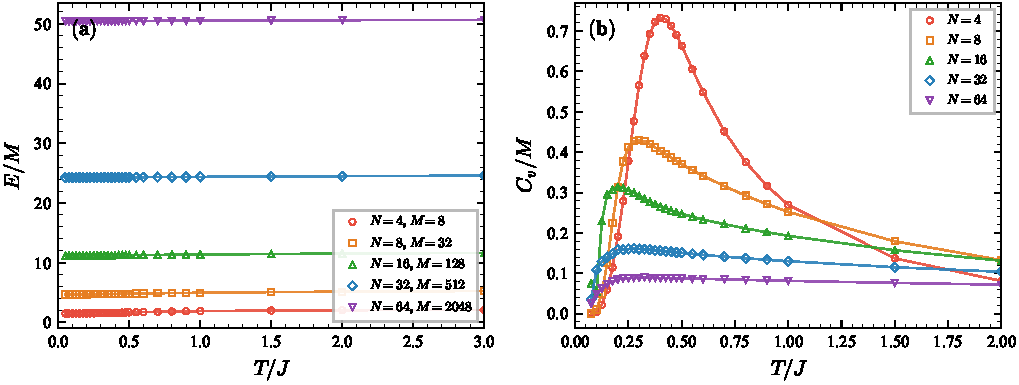
\includegraphics[width=\linewidth]{../figures/fig5_halffilling.pdf}
  \caption{半填充 $M = N^2/2$。(a)~每个皇后的能量 $E/M$ 随 $N$ 增长，标度为 $\sim 5N/6$。
  (b)~每个皇后的比热 $C_v/M$：峰变窄，每个皇后的涨落随 $N$ 减小（自平均）。与 $M = N$ 情形（图~\ref{fig:cv}）的对比——后者 $C_v/M$ 收敛——突显了稀薄和稠密区域的定性差异。}
  \label{fig:half}
\end{figure}


%=====================================================================
\section{总结}
\label{sec:conclusions}
%=====================================================================

我们对皇后格点气体进行了统计力学研究，从 $N$-皇后问题的组合基态熵追踪到其有限温度热力学。主要发现如下：

\begin{enumerate}
\item 基态熵 $s_0 = \ln N - \gamma$ 与理想气体的 Sackur--Tetrode 公式具有相同的函数形式。每个几何排斥约束（列、主对角线、反对角线）大约移除每个皇后一个单位的熵，其中列约束恰好消耗 1 个单位（Stirling 修正），两组对角线约束共消耗 $\gamma - 1 \approx 0.94$ 个单位。

\item 在 $T \to \infty$ 时，每皇后能量收敛到 $E/M = 5/3$，分解为行、列和两组对角线族的 $1/2 + 1/2 + 1/3 + 1/3$。每个贡献可从泊松占据统计推导：均值为 $\mu = 1$ 的线给出 $1/2 = \mu^2/2$，变化占据数的对角线给出 $1/3 = \int_0^1 \mu^2\,d\mu$。

\item 每皇后比热 $C_v/M(T)$ 在 $N \to \infty$ 时收敛到 $T$ 的普适函数。峰值高度 $\approx 1.62$ 不发散，排除了热力学相变，并将交叉行为认定为有效能隙 $\Delta = J$ 的 Schottky 反常。

\item 修正泊松平均场理论——将每条攻击线视为独立的修正泊松变量——给出了 $E/M(T)$ 和 $C_v/M(T)$ 的解析表达式，重现蒙特卡洛数据的精度在 $2$--$7\%$ 以内。残余偏差是 $O(1)$ 的系统效应：每对攻击线通过共享格点产生 $O(1/N)$ 的关联，但 $O(N^2)$ 对这样的关联产生在 $N \to \infty$ 极限下持续存在的累积修正。更简单的熵加权平均场 [$C_v^{\max} = 4(1+\gamma)/e^2$] 由于误差的部分抵消，在峰值处达到 $1.4\%$ 的精度。

\item $C_v/T$ 的热力学积分恢复了基态熵，偏差在 $2\%$ 以内，提供了非平凡的自洽性检验。该检验连接了三个独立要素：Simkin 组合公式、高温熵的 Stirling 近似、以及跨越整个温度范围的蒙特卡洛比热数据。

\item 在半填充（$M = N^2/2$）时，$E \sim N^3$，系统表现出自平均：每皇后比热 $C_v/M$ 随 $N$ 递减，因此相对能量涨落在热力学极限下消失。这与 $M = N$ 情形中 $C_v/M$ 收敛到非零函数形成对比，反映了高密度下每个皇后广延数量级（$O(N)$）的相互作用。

\end{enumerate}

这些结果将皇后格点气体确立为一个模型系统，其组合和热力学方面可在统一框架下研究。$N$-皇后熵与 Sackur--Tetrode 公式之间的结构对应、平均场理论的解析可处理性、以及稀薄和稠密填充区域之间丰富的交叉现象学，使该模型成为组合数学、统计力学和约束满足交叉领域中引人注目的试验场。

未来方向包括平行回火以访问更低温度、Schottky 交叉的有限尺寸标度理论、以及用副本重叠统计量探测解空间结构。


%=====================================================================
\begin{thebibliography}{30}

\bibitem{Bezzel1848}
M.~Bezzel,
Schachfreund, Berliner Schachzeitung \textbf{3}, 363 (1848).

\bibitem{Simkin2022}
M.~Simkin,
The number of $n$-queens configurations,
Adv.\ Math.\ \textbf{410}, 108735 (2022).

\bibitem{Bowtell2023}
C.~Bowtell and P.~Keevash,
The $n$-queens problem,
Ann.\ Math.\ \textbf{197}, 1 (2023).

\bibitem{Luria2021}
Z.~Luria and M.~Simkin,
New bounds on the number of $n$-queens configurations,
arXiv:2107.13460 (2021).

\bibitem{Nobel2023}
A.~Nobel, A.~Agrawal, and S.~Boyd,
Computing tighter bounds on the $n$-queens constant via Newton's
method,
Optim.\ Lett.\ \textbf{17}, 1229 (2023).

\bibitem{Reif1965}
F.~Reif,
\textit{Fundamentals of Statistical and Thermal Physics}
(McGraw-Hill, New York, 1965).

\bibitem{Knuth2022}
D.~E.~Knuth,
\textit{The Art of Computer Programming}, Vol.~4B
(Addison-Wesley, 2022), Sec.~7.2.2.

\bibitem{Zhang2009}
C.~Zhang and J.~Ma,
Counting solutions for the $N$-queens and Latin-square problems by
efficient Monte Carlo simulations,
Phys.\ Rev.\ E \textbf{79}, 016703 (2009).

\bibitem{Polson2024}
N.~Polson and V.~Sokolov,
Counting $N$ queens,
arXiv:2407.08830 (2024).

\bibitem{Mezard2009}
M.~M\'ezard and A.~Montanari,
\textit{Information, Physics, and Computation}
(Oxford University Press, Oxford, 2009).

\bibitem{Krzakala2007}
F.~Krzaka{\l}a, A.~Montanari, F.~Ricci-Tersenghi,
G.~Semerjian, and L.~Zdeborov\'a,
Gibbs states and the set of solutions of random constraint
satisfaction problems,
Proc.\ Natl.\ Acad.\ Sci.\ USA \textbf{104}, 10318 (2007).

\bibitem{Kawasaki1966}
K.~Kawasaki,
Diffusion constants near the critical point for time-dependent Ising
models.\ I,
Phys.\ Rev.\ \textbf{145}, 224 (1966).

\bibitem{Metropolis1953}
N.~Metropolis, A.~W.~Rosenbluth, M.~N.~Rosenbluth, A.~H.~Teller,
and E.~Teller,
Equation of state calculations by fast computing machines,
J.~Chem.~Phys.\ \textbf{21}, 1087 (1953).

\bibitem{Efron1982}
B.~Efron,
\textit{The Jackknife, the Bootstrap, and Other Resampling Plans}
(SIAM, Philadelphia, 1982).

\bibitem{Binder1997}
K.~Binder and D.~W.~Heermann,
\textit{Monte Carlo Simulation in Statistical Physics}
(Springer, Berlin, 5th ed., 2010).

\bibitem{Mezard1987}
M.~M\'ezard, G.~Parisi, and M.~A.~Virasoro,
\textit{Spin Glass Theory and Beyond}
(World Scientific, Singapore, 1987).

\end{thebibliography}

\end{document}
